\documentclass[12pt]{My_preprint}

%%%%%%%%%%%%%%%%%%%%%%%%%%%%%%%%%%%%%%%%%%%%%%%%%%%%%%%%%%%%%%%%%%%%%%%%%%%%%%%

%%%%%%%%%%%%%%%%%%%%%%%%%%%%%%% Title & Author %%%%%%%%%%%%%%%%%%%%%%%%%%%%%%%%


%\title{The hybrid model for arbitrary dispersed multiphase flows with surface properties}
\title{Averaged equations for spheroidal particles  }

\author[1]{Nicolas Fintzi}
\author[1]{Jean-Lou Pierson}
% \author[2]{Stephane Popinet}
% \author[2]{Daniel Lhuillier}
\affil[1]{IFP Energies Nouvelles, Rond-point de l’changeur de Solaize, 69360 Solaize}
% \affil[2]{Sorbonne Université, Institut Jean le Rond d'Alembert, 4 place Jussieu, 75252 PARIS CEDEX 05, France}


\begin{document}

\maketitle

\begin{abstract}
    In this work we propose to derive an averaged set of equations for dilute suspension of spheroidal particles. 
    We consider small but non-zero effects of inertial, such that $Re<1$, where $Re$ is the Reynolds number based on the relative velocity. 
    The Reynolds number based on shear, and rotational motion are assumed to be small.
    The closure are derived using the methodology of \citet{brenner1963resistance} within the Stokes flow hypothesis. 
    Then the results are extended to slightly inertial flow using the reciprocal theorem based on the stokes flow solution. 
\end{abstract}


\section{Dynamic of a single particle}

We consider a spheroidal particle, which volume is described by the vectors, 
\begin{equation}
    \textbf{r} 
    = r [1 + \epsilon \textbf{H}:\textbf{S}(\textbf{n})]\textbf{e}_r,
    = r [1 + f]\textbf{n},
\end{equation}

where $r\in [0;1]$, $\textbf{S} = \textbf{nn} - \frac{1}{3}\bm\delta$ is the surface spherical harmonics of order $2$, and \textbf{H} the second order tensor quantifying the deformation of the spheroidal particle (see \citet{nadim1996concise} for a geometrical interpretation).  
$\epsilon\ll 1$ is a very small parameter. 

To understand how $\textbf{H}$ is related to the three radius of the particle we use the relation, 
\begin{equation}
    \int_{V} \textbf{rr} dV = (\frac{4\pi a^2}{3}) a^2/5(\bm\delta+ 2\epsilon \textbf{H})
\end{equation}
Also, by direct calculation in the principal axis of the spheroid, noted $\textbf{p}_n$ one obtain, 
\begin{equation}
    \int \textbf{rr} dV =  \frac{4\pi a^3}{3} ((a_1/a)^2 \textbf{p}_1 \textbf{p}_1+ (a_2/a)^2\textbf{p}_2 \textbf{p}_2 + (a_3/a)^2\textbf{p}_3 \textbf{p}_3)a^2/5
\end{equation}
see \url{https://mathworld.wolfram.com/Ellipsoid.html}. 
Hence, our definition of \textbf{H} is, 
\begin{equation}
    2\epsilon \textbf{H}= (a_1/a)^2 \textbf{p}_1 \textbf{p}_1+ (a_2/a)^2\textbf{p}_2 \textbf{p}_2 + (a_3/a)^2\textbf{p}_3 \textbf{p}_3 - \bm\delta,
\end{equation}
one may eventually express $\textbf{p}_3$ as $\textbf{p}_1 \times \textbf{p}_2$ hence only to independent vector constitutes $\textbf{H}$. 
Note also that the isotropic part vanish in the torque expression given below. 


For instance, we discard the effect of inertia. 
In this case the equations governing the disturbance pressure and velocity fields $(p,\textbf{u})$, around the isolated particle are, 
\begin{align}
    \div \textbf{u}= 0&& \grad^2 \textbf{u}=\grad p\\
    \textbf{u} = \textbf{u}_r\;\; \forall r = 1+\epsilon \textbf{H}:\textbf{S} 
    && \lim_{r\to \infty} (\textbf{u},p) = (\textbf{0},0)
\end{align}
where $\textbf{u}_r = \textbf{U}-   \textbf{u}_p$, with \textbf{U} the background velocity field, and $\textbf{u}_p$ the center of mass velocity field. 

Because we cannot apply these boundaries condition directly we express any of the above function as a taylor expansion in terms of $\epsilon$ such that, any tensor \textbf{F} can be expressed as, 
\begin{equation}
    \textbf{F}
    = \ps{0}{\textbf{F}}
    + \epsilon \ps{1}{\textbf{F}}
    + O(\epsilon^2)
\end{equation}
Then, any function to be evaluated on the droplet interface might be written as, 
\begin{equation}
    \textbf{F}(r=1+\epsilon f)
    % =
    % \textbf{F}|_{r=1}
    % + \epsilon f \frac{\partial \textbf{F}}{\partial r}|_{r=1}
    =
    \ps{0}{\textbf{F}}|_{r=1}
    + \epsilon \left[\ps{1}{\textbf{F}}
    + f \frac{\partial\ps{0}{\textbf{F}}}{\partial r}\right]_{r=1}
    + O(\epsilon)
    =
    \ps{0}{\textbf{F}}|_{r=1}
    + \epsilon \left[\ps{1}{\textbf{F}}
    + f (\textbf{n}\cdot \grad) \ps{0}{\textbf{F}} \right]_{r=1}
    + O(\epsilon). 
\end{equation}
Doing so one can solve a stokes problem for $\ps{0}{\textbf{u}}$ in terms of $\textbf{u}_r$ and of $\ps{1}{\textbf{u}}$ in terms of $\textbf{H}$. 
Note that at this stage $\textbf{u}_r$ is arbitrary, and can represent uniform, linear or quadratic flow. 

Once these solutions are obtained one can use the reciprocal theorem to find out the effect of inertia on the first moment on a translating spheroidal particle. 
This is done by applying the reciprocal theorem between $Eq(\textbf{u}^{Re})$ which are the equations governing the inertial flow, and $Eq(\textbf{u})$ which represent the stokes flow around that particle. 
In the configuration where $Eq(\textbf{u}^{Re})$ represent uniform translation of the spheroidal particle and $Eq(\textbf{u})$ a linear flow around the deformed droplet in stokes flow, one obtain the expression, 
\begin{equation}
    \intS[p]{\textbf{r}\bm\sigma^{Re}\cdot \textbf{n}}
    % - \intO[i]{2\textbf{e}_i}
    % - (1-\lambda) \intO[p]{(\textbf{u}_{i} + \textbf{u}_r)\cdot \grad^2 \hat{\textbf{u}}}
    % + \intS[p]{2(\textbf{u}_{i} + \textbf{u}_r)\cdot \hat{\textbf{b}}}
    % \\
    =
    % \intS[p]{\textbf{u}_{r}\cdot \textbf{S}^{(2)}_{o}\cdot \textbf{n}}
    % - \intO[i]{\textbf{S}^{(2)}_{i}:\grad\textbf{u}}
    % - (1-\lambda) \intO[p]{(\textbf{U}_{i}^{(2)} + \textbf{r}\bm\delta) \cdot \grad^2 \textbf{u} }\\ 
    % + \intS[p]{2(\textbf{U}_{i}^{(2)} + \textbf{r}\bm\delta) \cdot  \textbf{b}}
    % + \zeta Re \intO{(\textbf{U}_{i}^{(2)} + \textbf{r}\bm\delta)\cdot \textbf{f}_{i}} 
    \ldots + Re\intO[o]{\textbf{U}_{o}^{(2)}\cdot \textbf{f}_{o}},
    = \ldots + Re\intO[o]{\textbf{U}_{o}^{(2)}\cdot (\textbf{U}^{(1)} + \bm\delta)\cdot \grad \textbf{U}^{(1)}} : \textbf{u}_r\textbf{u}_r,
    \label{eq:first_mom}
\end{equation}
where $\textbf{U}_{o}^{(2)}\cdot \grad \textbf{U}$ is the disturbance velocity field generated by a spheroidal particle immersed in pure linear flow, and $\textbf{U}_{o}^{(2)}\cdot \grad \textbf{u}_r$ the disturbance field of the same particle immersed in a uniform flow of relative velocity $\textbf{u}_r$. 
The terms represented by the $\ldots$ represent the other non-inertial contribution partially  given by \citet{brenner1963resistance} (he does not provide the Stresslet). 

Carrying the computation and retaining only the term proportional to $Re \epsilon$ (neglecting the $\epsilon^2$ terms), yields, 

\begin{align}
    M_{ij}=
    \frac{1}{2}\intS[p]{[ r_i (\bm\sigma^{Re}\cdot \textbf{n})_j- r_j (\bm\sigma^{Re}\cdot \textbf{n})_i]}
    =
    \ldots
      Re \epsilon \pi
    \frac{29}{40}[H_{jk}(\textbf{u}_r)_i - H_{ik}(\textbf{u}_r)_j ] (\textbf{u}_r)_k
    \label{eq:first_mom}
\end{align}
where $\textbf{R}$ is the resistance matrix of the spheroidal particle in stokes flow. 

Then the torque may be obtained as, 
\begin{equation}
    T_l = - \frac{1}{2}\epsilon_{lij}M_{ij}
    % =- \frac{1}{2}\epsilon_{lij} Re \epsilon \pi 
    % \frac{29}{40}[H_{jk}(\textbf{u}_r)_i - H_{ik}(\textbf{u}_r)_j ] (\textbf{u}_r)_k
    =- \frac{1}{2} Re \epsilon \pi 
    \frac{29}{40} \epsilon_{lij}H_{jk}(\textbf{u}_r)_i  (\textbf{u}_r)_k
    =\tb{\pm(\frac{1}{2} ?)} Re \epsilon \pi 
    \frac{29}{40} (\textbf{u}_r\times \textbf{H})_{lk}  (\textbf{u}_r)_k
\end{equation}

\tb{Voir \citet[p.29]{guazzelli2011} pour une definitions des pseudo vecteur, car le $1/2$ me semble un peu arbitraire. Et surtout voir quelle convention utilise Cox. Je crois que pour le signe c'est aussi une affaire de right-hand rule ou non donc a verifier }
To make the results dimensional multiply the above expression by $a^2 \mu_f U$ where $a$ is the mean radius of the sphere of same volume. Because upon changing $\textbf{H}$ the volume does not change. 


\section{Note JL}
\subsection{Introduction}
The shape of a nearly spherical particle (all the distances are normalised by $a$) may be written as (Nadim \& Stone (1991)),
\begin{equation}
  r_s 
  = [1 + \varepsilon f (\textbf{e}_r)],
\end{equation}
where $\varepsilon$ is a small parameter and $\textbf{e}_r$ is the unit vector normal to the sphere.
Then, the shape function is expanded in a series of surface spherical harmonic as
\begin{equation}
f(\textbf{e}_r) = \sum_{n=1}^{\infty}\textbf{H}^{(n)}:\textbf{S}^{(n)} (\textbf{e}_r)
\end{equation}
where $\textbf{H}^{(n)}$ are $n$-th order tensor and $\textbf{S}^{(n)}$ are the $n$-th surface spherical harmonic.
\JL{
Can we include $\textbf{H}^{(1)}$ to bend the particle or $\textbf{H}^{(3)}$ to lose a symmetry plane ?
 }
%Since at leading order $\textbf{n}  = \textbf{e}_$ one obtain%$ where $\textbf{e}$ is the unit vector normal to the sphere ($a$ is the radius of the sphere)
Any points within the particles may be desribed with,
\begin{equation}
  \textbf{r} 
  = r[1 + \epsilon f(\textbf{e}_r)]\textbf{e}_r,
  %= a [1 + \epsilon \textbf{H}:\textbf{S}(\textbf{e})]\textbf{e},
\end{equation}
where $r$ is the spherical radial coordinate.
From this definition various quantities may be obtained such as the second-order moment of mass defined as
\begin{align}
  \textbf{M}_p
  &=
  \int_{V}{\textbf{rr}}dV \\
  &=
  \int_{\text{unit sphere}}{r^4 (1+ 5\varepsilon f(\textbf{e}_r)) \textbf{e}_r \textbf{e}_r \sin\theta  dr d\theta d\varphi} + \mathcal{O}(\varepsilon^2) \\
  &= 
  \frac{4\pi}{15} \bm \delta + 5\varepsilon \int_{\text{unit sphere}}{r^4  f(\textbf{e}_r) \textbf{e}_r \textbf{e}_r \sin\theta  dr d\theta d\varphi} + \mathcal{O}(\varepsilon^2) 
\end{align}
since $dV = (1+ \varepsilon f)^3r^2\sin\theta  dr d\theta d\varphi$ and $\int_{\text{unit sphere}} \textbf{e}_r \textbf{e}_r \sin\theta  d\theta d\varphi = 4\pi/3 \bm \delta$.
%Attention, il faut distinguer le r vecteur qui represente la distance au centre du r vecteur qui reprendre la surface deformeee.
%OK integrer jusqu'a la surface deformee avec l'expression du vecteur deformee.

\subsection{Second-order harmonic deformation}
We assume that the shape function is given by $f = \textbf{H}^{(2)}:\textbf{S}^{(2)}$ where $\textbf{S}^{(2)} = \textbf{e}_r\textbf{e}_r - \frac{1}{3}\bm\delta$ is the surface spherical harmonics of order $2$.
\JL{without loss of generality since $\textbf{S}^{(2)}$ is symmetric we assume that $\textbf{H}^{(2)}$ is symmetric.}
$\textbf{H}^{(2)}:\textbf{S}^{(2)}$ is also traceless by mass conservation.
Let's compute (we disregard the isotropic part which vanish)
%\begin{equation}
%  \int_{V} \textbf{rr} dV = \int_{Vsphere} r^2\textbf{ee} dV + 2 a^2 \epsilon \int_{V} (\textbf{H}:\textbf{S}) \textbf{ee} dV
%\end{equation}
\begin{align}
  \textbf{M}_p
  &=
  \frac{4\pi}{15}\bm\delta+
  5 \varepsilon \textbf{H}^{(2)}: \int_{\text{unit sphere}}{r^4 \textbf{e}_r \textbf{e}_r \textbf{e}_r \textbf{e}_r }\sin\theta dr d\theta d\varphi\\
  &=
  \frac{4\pi}{15}[\bm\delta+
  \varepsilon \textbf{H}^{(2)}_{kl}: (
      \bm\delta_{ij}
      \bm\delta_{kl}
      +\bm\delta_{ik}
      \bm\delta_{jl}
      +\bm\delta_{il}
      \bm\delta_{jk}
  )
  ]\\
  &=
  \frac{4\pi}{15}[\bm\delta+
  2 \varepsilon \textbf{H}^{(2)}
  ]
\end{align}
since $\int_{\text{unit sphere}} \textbf{e}_r \textbf{e}_r \textbf{e}_r \textbf{e}_r\sin\theta  d\theta d\varphi = 4\pi/15 (
  \bm\delta_{ij}
  \bm\delta_{kl}
  +\bm\delta_{ik}
  \bm\delta_{jl}
  +\bm\delta_{il}
  \bm\delta_{jk}
)$ and $\textbf{H}^{(2)}:\bm \delta =0$ (volume conservation).

By direct calculation in the principal axis of the ellispoid, noted $\textbf{p}_n$ one obtain, in dimensional form
\begin{equation}
    \int \textbf{rr} dV =  \frac{4\pi}{15}a_pa_qa_n (a_p^2 \textbf{p} \textbf{p}+ a_q^2\textbf{q} \textbf{q} + a_n^2\textbf{n} \textbf{n})
\end{equation}
In the limit of small deformation $a_p = a (1+\epsilon \alpha)$, $a_q = a (1+\epsilon \beta)$, $a_n = a (1+\epsilon \gamma)$,
\begin{equation}
  \int \textbf{rr} dV =  \frac{4\pi}{15} (\bm \delta + \epsilon \left[(3\alpha +\beta +\gamma) \textbf{p} \textbf{p}+ (\alpha +3\beta +\gamma)\textbf{q} \textbf{q} + (\alpha +\beta +3\gamma)\textbf{n} \textbf{n}\right]) + \mathcal{O}(\varepsilon^2)
\end{equation}
Then due to the volume conservation, $\gamma = -\alpha -\beta$ and we finally obtain,
\begin{equation}
\textbf{H}^{(2)} = \alpha \textbf{p} \textbf{p} + \beta \textbf{q} \textbf{q} - (\alpha + \beta) \textbf{n} \textbf{n} 
\end{equation}
\subsection{Reciprocal theorem}
\begin{align}
  M_{ij}=
  \frac{1}{2}\intS[p]{[ r_i (\bm\sigma^{Re}\cdot \textbf{n})_j- r_j (\bm\sigma^{Re}\cdot \textbf{n})_i]}
  =
  \ldots
    Re \epsilon \pi
  \frac{29}{40}[H_{jk}(\textbf{u}_r)_i - H_{ik}(\textbf{u}_r)_j ] (\textbf{u}_r)_k
  \label{eq:first_mom}
\end{align}

Since, $T _ l  = \epsilon _{lij}   M_{ij}$ one obtain,

\begin{equation}
  T _ l = - \frac{29 }{20} \pi Re \epsilon  (\epsilon _{lij}H_{jk}(\textbf{u}_r)_i)(\textbf{u}_r)_k
\end{equation}
which may alo be rewritten as,
\begin{equation}
  \bm T  = - \frac{29 }{20} \pi Re \epsilon  (\alpha \bm u \times \bm p u_p +\beta\bm u \times \bm q u_q-(\alpha+\beta)\bm u \times \bm n u_n )
\end{equation}
Then,
\begin{align}
  T_p  &=  \frac{29 }{20} \pi Re \epsilon  (\alpha +2\beta) u_q u_n \\
  T_q  &=  -\frac{29 }{20} \pi Re \epsilon  (2\alpha +\beta) u_p u_n,\\
  T_n  &=  \frac{29 }{20} \pi Re \epsilon  (\alpha -\beta) u_p u_q
\end{align}





\section{Quasi-steady motion of a settling ellipsoid ($x$ convention) WRONG}
The Euler angle defined here are the one defined by Goldstein p 146 ($x$ convention)
\subsection{Quasi-steady balance}
%We consider an ellipsoidal particle settling under gravity with dimensionless velocity $\bm v$ and dimensionless angular velocity $\bm \omega$ in a fluid at rest at infinity. 
%We consider a quasi-steady balance, and we assume that the unsteady term in the Navier Stokes equations is much smaller than the dvective term . 
%Since the characteristic time scale is given by the particle we have $\tau \sim \omega ^{-1}$
%Then the quasi-steady assumption is justified as long as $\omega a / v \ll 1$ where $\omega$ is the characteristic angular velocity,  \citep{cox1965,pierson2023}.
%$a$ is the chracteristics size of the body and $v$ its charcatetistic velocity.
%This assumption may also be rewritten as $Re _\omega /\Re _p  \ll 1$ where $Re_p = \rho  v a/\mu$ and $Re _\omega = \rho \omega a^2 /\mu$.
%As demonstrated in the previous sections, under this limit the load on a settling ellipsoidal particles reduces to,
We consider the sedimentation of an ellipsoidal particle under gravity, characterized by the dimensionless translational velocity $\mathbf{v}$ and angular velocity $\boldsymbol{\omega}$, in a fluid that is quiescent at infinity. 
The analysis is conducted under a quasi-steady approximation, where the unsteady contribution to the Navier-Stokes equations is assumed to be much smaller than the convective term. 
The relevant timescale is determined by the particle rotational dynamics, such that $\tau \sim \omega^{-1}$ \citep{cox1965,pierson2023}.
Accordingly, the quasi-steady assumption is valid provided that $\omega a/v \ll 1,$
where $\omega$ denotes the characteristic angular velocity, $a$ the characteristic particle dimension, and $v$ the characteristic settling velocity.
This condition may be recast in terms of Reynolds numbers as $Re_\omega/Re_p \ll 1$,
with $Re_p = \rho v a / \mu$ the translational Reynolds number and $Re_\omega = \rho \omega a^2 / \mu$ the rotational Reynolds number.
As demonstrated in the previous section, in this regime the hydrodynamic load acting on a settling ellipsoidal particle reduces to (check sign of the inertial torque),
\begin{align}
    \bm F &= - \mathbb{A} \cdot \bm v - Re_p (...)  \\
    \bm T &= - \mathbb{C} \cdot \bm \omega + Re_p\mathbb{N} : \hat{\bm  v} \hat{\bm v}
\end{align}

Then the dimensionless equations of motion expressed in the laboratory reference frame but axes rotating with the body read,
\begin{align}
    \bar{\rho} Re_\omega \left(\mathbb{I}\cdot\frac{\mathrm{d}\bm v}{\mathrm{d}t} +\bm \omega \times (\mathbb{I}\cdot \bm v) \right) &= - \mathbb{A} \cdot \bm v + Re_p (...)+ \bm F_b,
    \label{eq:forcebal} \\
    \bar{\rho} Re_\omega \left(\mathbb{J}\cdot\frac{\mathrm{d}\bm \omega}{\mathrm{d}t} + \bm \omega \times (\mathbb{J}\cdot  \bm \omega)\right)  &= - \mathbb{C} \cdot \bm \omega + \frac{Re _p ^2}{Re_\omega}\mathbb{N} : \hat{\bm  v} \hat{\bm v},
    \label{eq:torquebal}
\end{align}
where $\bm F_b = (m - \rho V) \mathbf{g}/(\mu v a)$ is the dimensionless buoyancy force, $m$ and $V$ are respectively the mass and volume, $\mathbb{I}$ is the identity matrix, $\mathbb{J}$ is the dimensionless inertia tensor.
%\begin{align}
%    m \left(\mathbb{I}\cdot\frac{\mathrm{d}\bm v}{\mathrm{d}t} +\bm \omega \times (\mathbb{I}\cdot \bm v) \right) &= \bm F+ (m - \rho V) \mathbf{g},
%    \label{eq:forcebal} \\
%    \mathbb{J}\cdot\frac{\mathrm{d}\bm \omega}{\mathrm{d}t} + \bm \omega \times (\mathbb{J}\cdot  \bm \omega)  &= \bm T,
%    \label{eq:torquebal}
%\end{align}
%, coupling between rotation and translation.
We assume that $Re_\omega \ll Re _ p \ll 1$ (\textit{i.e.} $\omega a /v \ll 1$) such that $ Re _p ^2 /Re_\omega \sim 1$.
We also consider the particle to fluid density ratio to be of order one (such that $\bar{\rho} Re_\omega \ll 1$).
Then one is left with,
\begin{align}
    \bm 0 &= - \mathbb{A} \cdot \bm v + \bm F_b,
    \label{eq:forcebal1} \\
    \bm 0 &= - \mathbb{C} \cdot \bm \omega + \frac{Re _p ^2}{Re_\omega}\mathbb{N} : \hat{\bm  v} \hat{\bm v},
    \label{eq:torquebal1}
\end{align}
%(To be justified thanks to Cox 1965 analysis - valid only for $Ga \ll 1$)
%In addition we disregard all term in $\mathcal O(Re)$ in the force balance, and all term quadratic in the angular velocity in the angular momentum balance.
Then, still in axes rotating with the particle, one is left to,

\begin{align}
    0 &= -A_{pp} v_p - F_b\ \sin \psi \sin \theta, \label{eq:vp}\\
    0 &= -A_{qq} v_q - F_b\cos \psi \sin \theta,
\label{eq:vq} \\
   0 &= -A_{nn} v_n - F_b\cos \theta,
\label{eq:vn}
\end{align}
and
\begin{align}
    0 &= -C_{pp} \omega_p + N_{pqn} v_q v_n, \label{eq:omp}\\
    0 &= -C_{qq} \omega_q + N_{qpn} v_p v_n, \label{eq:omq} \\
   0 &= -C_{nn} \omega_n + N_{npq} v_p v_q,\label{eq:omn}
\end{align}
with,
\begin{align}
    \omega_p &= \dot \phi \sin \psi \sin \theta +  \dot \theta \cos \psi, \\
    \omega_q &= \dot \phi \cos \psi \sin \theta -  \dot \theta \sin \psi, \\
    \omega_n &= \dot \phi \cos \theta +  \dot \psi, \\
\end{align}
Then,
\begin{align}
    \dot \phi \sin \psi \sin \theta +  \dot \theta \cos \psi &= \frac{N_{pqn}}{C_{pp}} \frac{F_b^2}{A_{qq} A_{nn}}\cos \psi \sin \theta\cos \theta, \\
    \dot \phi \cos \psi \sin \theta -  \dot \theta \sin \psi &= \frac{N_{qpn}}{C_{qq}} \frac{F_b^2}{A_{pp} A_{nn}}\sin \psi \sin \theta\cos \theta, \\
    \dot \phi \cos \theta +  \dot \psi &= \frac{N_{npq}}{C_{nn}}\frac{F_b^2}{A_{pp} A_{qq}}\sin \psi \cos \psi (\sin \theta) ^2,\\
\end{align}
where $F_b = (m-\rho V)g/(\mu v a)$.
Then after straightforward algebra,
\begin{align}
    \dot \phi  &= \sin \psi \cos \psi  \cos \theta F_b^2 \left(\frac{N_{pqn}}{C_{pp}A_{qq} A_{nn}}+\frac{N_{qpn}}{C_{qq}A_{pp} A_{nn}}\right), \\
    \dot \theta  &= \cos \theta \sin \theta F_b^2 \left(\frac{N_{pqn}}{C_{pp}A_{qq} A_{nn}} - \frac{N_{qpn}}{C_{qq}A_{pp} A_{nn}}\right), \\
    \dot \psi   &= -\sin \psi \cos \psi F_b^2 \left((\cos \theta)^2\left(\frac{N_{pqn}}{C_{pp}A_{qq} A_{nn}}+\frac{N_{qpn}}{C_{qq}A_{pp} A_{nn}}\right)-\frac{N_{npq}}{C_{nn}}\frac{F_b^2}{A_{pp} A_{qq}}(\sin \theta) ^2\right).
\end{align}
%From the last set of equations one may identify the following fixed points $\{\theta =0,  \psi = 0\}$, $\{\theta =0,  \psi = \phi/2\}$, $\{\theta =\pi/2,  \psi = 0\}$, $\{\theta =\pi/2,  \psi = \phi/2\}$.
%Before investigating it further let us repeat Cox (1965) analysis.
From the final set of equations, the following fixed points can be identified:
$\{\theta = 0, \, \psi = 0\}$, $\{\theta = 0, \, \psi = \pi/2\}$, $\{\theta = \pi/2, \, \psi = 0\}$, and $\{\theta = \pi/2, \, \psi = \pi/2\}$.
Before proceeding further, let us first revisit the analysis of Cox (1965) for a spheroid.

\JL{wrong because not the good convention}
\subsection{Orientation of a spheroid}



For a spheroid parametrized as defined in section V,  $N_{npq} = 0$  and $N_{pqn} = - N_{qpn}$, $A = A_{pp} =A_{qq}$, $C = C_{pp} =C_{qq}$. 
Then, 
\begin{align}
    \dot \theta  &= 2\cos \theta \sin \theta \frac{N_{pqn}F_b^2}{CA A_{nn}}, \\
\end{align}
$A_{pp}, ...$ coefficients are all postive. Same for $C_{pp}, ...$. 
Then the orientation stability only depends on the sign of $N_{pqn}$, which itself depends on the shape of the spheroid ($i.e.$ prolate or oblate).
Indeed linearizing the previous equation around $\theta =0$ (or $\theta =\pi/2$) one gets,
\begin{align}
 \theta &= 0 \quad   \dot \theta  =  2\theta \frac{N_{pqn}F_b^2}{CA A_{nn}} \quad \text{stable if $N_{pqn}< 0$}, \\
 \theta &= \frac{\pi}{2} \quad   \dot \theta  =  -2\theta \frac{N_{pqn}F_b^2}{CA A_{nn}} \quad \text{stable if $N_{pqn}> 0$},.
\end{align}

For a spheroid with a small aspect ratio, using $C = 8\pi$, $A = 6\pi$, $A_{nn} = 6\pi$, $F_b^2$, and $N_{pqn} = \frac{29}{20}\pi \varepsilon$ (prolate if $\varepsilon >0$ ?), our results appear to differ from Cox by a factor of $3/2$.

%Then if $N_{pqn}$ is positive ...

\subsection{Orientation of an ellipsoid}
We linearize the governing equations around the fixed points.
 
\subsubsection{$\{\theta = 0, \, \psi = 0\}$}
\begin{align}
    \dot \theta  &=  \theta F_b^2 \left(\frac{N_{pqn}}{C_{pp}A_{qq} A_{nn}} - \frac{N_{qpn}}{C_{qq}A_{pp} A_{nn}}\right) \quad \text{stable if $\frac{N_{pqn}}{C_{pp}A_{qq} A_{nn}}$} <\frac{N_{qpn}}{C_{qq}A_{pp} A_{nn}}, \\
    \dot \psi   &=  \psi F_b^2 \left(\frac{N_{pqn}}{C_{pp}A_{qq} A_{nn}}+\frac{N_{qpn}}{C_{qq}A_{pp} A_{nn}}\right)\text{stable if $\frac{N_{pqn}}{C_{pp}A_{qq} A_{nn}}  < -\frac{N_{qpn}}{C_{qq}A_{pp} A_{nn}}$}.
\end{align}
\subsubsection{$\{\theta = 0, \, \psi = \pi/2\}$}
\begin{align}
    \dot \theta  &=  \theta F_b^2 \left(\frac{N_{pqn}}{C_{pp}A_{qq} A_{nn}} - \frac{N_{qpn}}{C_{qq}A_{pp} A_{nn}}\right) \quad \text{stable if $\frac{N_{pqn}}{C_{pp}A_{qq} A_{nn}}$} <\frac{N_{qpn}}{C_{qq}A_{pp} A_{nn}}, \\
    \dot \psi   &=  -\psi F_b^2 \left(\frac{N_{pqn}}{C_{pp}A_{qq} A_{nn}}+\frac{N_{qpn}}{C_{qq}A_{pp} A_{nn}}\right) \quad \text{stable if $\frac{N_{pqn}}{C_{pp}A_{qq} A_{nn}}  > -\frac{N_{qpn}}{C_{qq}A_{pp} A_{nn}}$}.
\end{align}
\subsubsection{$\{\theta = \pi/2, \, \psi = 0\}$}
\begin{align}
    \dot \theta  &=  -\theta F_b^2 \left(\frac{N_{pqn}}{C_{pp}A_{qq} A_{nn}} - \frac{N_{qpn}}{C_{qq}A_{pp} A_{nn}}\right)\quad \text{stable if $\frac{N_{pqn}}{C_{pp}A_{qq} A_{nn}}$} >\frac{N_{qpn}}{C_{qq}A_{pp} A_{nn}}, \\
    \dot \psi   &= -\psi F_b^2 \left(\frac{N_{npq}}{C_{nn}}\frac{F_b^2}{A_{pp} A_{qq}}\right)\quad \text{stable if $\frac{N_{npq}}{C_{nn}}\frac{F_b^2}{A_{pp} A_{qq}}>0$}.
\end{align}
\subsubsection{$\{\theta = \pi/2, \, \psi = \pi/2\}$}
\begin{align}
    \dot \theta  &=  -\theta F_b^2 \left(\frac{N_{pqn}}{C_{pp}A_{qq} A_{nn}} - \frac{N_{qpn}}{C_{qq}A_{pp} A_{nn}}\right)\quad \text{stable if $\frac{N_{pqn}}{C_{pp}A_{qq} A_{nn}}$} >\frac{N_{qpn}}{C_{qq}A_{pp} A_{nn}}, \\
    \dot \psi   &= \psi F_b^2 \left(\frac{N_{npq}}{C_{nn}}\frac{F_b^2}{A_{pp} A_{qq}}\right)\quad \text{stable if $\frac{N_{npq}}{C_{nn}}\frac{F_b^2}{A_{pp} A_{qq}}<0$}.
\end{align}

\subsubsection{Discussion}

The $\theta$ stability depends on the sign of
\begin{equation}
\frac{N_{qpn}}{C_{qq} A_{pp} A_{nn}} - \frac{N_{pqn}}{C_{pp} A_{qq} A_{nn}} .
\end{equation}
However, the values of $N_{qpn}$ and $N_{pqn}$ are not known for ellipsoidal particles of arbitrary shape.
Moreover, the stability of $\psi$ also depends on the value of $\theta$.
In the following, we focus on an ellipsoid close to a spherical shape (see Section V), for which:

$$
N_{pqn} = \frac{29}{20}\pi \varepsilon, \quad
N_{qpn} = -\frac{29}{20}\pi \alpha \varepsilon, \quad
N_{npq} = \frac{29}{20}\pi (\alpha - 1)\varepsilon, \quad $$

$$
A_{pp} = 6\pi, \quad A_{qq} = 6\pi,  \quad A_{nn} = 6\pi ,
C_{pp} = 8\pi, \quad C_{qq} = 8\pi,  \quad C_{nn} = 8\pi .
$$

\subsubsection{$\{\theta = 0, \, \psi = 0\}$}

$\theta$ stable if $N_{pqn} < N_{qpn}$ or $\varepsilon < -\alpha \varepsilon$ which requires  $-1>\alpha$ if  $\varepsilon > 0$ or $-1 < \alpha$ if $\varepsilon < 0$ .\\
$\psi$ stable if $N_{pqn} < -N_{qpn}$ or $\varepsilon < \alpha \varepsilon$ which requires  $1<\alpha$ if  $\varepsilon > 0$ or $1 > \alpha$ if $\varepsilon < 0$


\subsubsection{$\{\theta = 0, \, \psi = \pi/2\}$}
$\theta$ stable if $N_{pqn} < N_{qpn}$ or $\varepsilon < -\alpha \varepsilon$ which requires  $-1>\alpha$ if  $\varepsilon > 0$ or $-1 < \alpha$ if $\varepsilon < 0$ .\\
$\psi$ stable if $N_{pqn} > -N_{qpn}$ or $\varepsilon > \alpha \varepsilon$ which requires  $1>\alpha$ if  $\varepsilon > 0$ or $1 < \alpha$ if $\varepsilon < 0$

\subsubsection{$\{\theta = \pi/2, \, \psi = 0\}$}
$\theta$ stable if $N_{pqn} > N_{qpn}$ or $\varepsilon > -\alpha \varepsilon$ which requires  $-1<\alpha$ if  $\varepsilon > 0$ or $-1 > \alpha$ if $\varepsilon < 0$ .\\
$\psi$ stable if $N_{npq}>0$ or $(\alpha - 1)\varepsilon > 0$ which requires  $1 <\alpha$ if  $\varepsilon > 0$ or $1 > \alpha$ if $\varepsilon < 0$

\subsubsection{$\{\theta = \pi/2, \, \psi = \pi/2\}$}
$\theta$ stable if $N_{pqn} > N_{qpn}$ or $\varepsilon > -\alpha \varepsilon$ which requires  $-1<\alpha$ if  $\varepsilon > 0$ or $-1 > \alpha$ if $\varepsilon < 0$ .\\
$\psi$ stable if $N_{npq}<0$ or $(\alpha - 1)\varepsilon < 0$ which requires  $1 >\alpha$ if  $\varepsilon > 0$ or $1 < \alpha$ if $\varepsilon < 0$

\subsection{Discussion}
In Bagheri's work, ellipsoidal particles are shown to adopt a stable orientation that maximizes their drag ?
In other words, the particle aligns such that the projected surface area on a plane perpendicular to the direction of gravity is maximized ?

Then from the above figure one may expect,

\begin{equation}
\varepsilon = 0.3, \alpha = 2 \quad \text{stable for $\theta = \pi/2, \psi =\pi /2$ ? check Mohsen results}
\end{equation}
Does it agree with our results :  Yes for $\theta $ No for $\psi$ 

\section{Quasi-steady balance $y$ convention}

\begin{align}
    0 &= -A_{pp} v_p + F_b\ \cos \psi \sin \theta, \label{eq:vp}\\
    0 &= -A_{qq} v_q - F_b\sin \psi \sin \theta,
\label{eq:vq} \\
   0 &= -A_{nn} v_n - F_b\cos \theta,
\label{eq:vn}
\end{align}
and
\begin{align}
    0 &= -C_{pp} \omega_p + N_{pqn} v_q v_n, \label{eq:omp}\\
    0 &= -C_{qq} \omega_q + N_{qpn} v_p v_n, \label{eq:omq} \\
   0 &= -C_{nn} \omega_n + N_{npq} v_p v_q,\label{eq:omn}
\end{align}
with,
\begin{align}
  \omega_p &= -\dot \phi \cos \psi \sin \theta +  \dot \theta \sin \psi, \\
  \omega_q &= \dot \phi \sin \psi \sin \theta +  \dot \theta \cos \psi, \\
  \omega_n &= \dot \phi \cos \theta +  \dot \psi, \\
\end{align}
Then,
\begin{align}
  -\dot \phi \cos \psi \sin \theta +  \dot \theta \sin \psi &= \frac{N_{pqn}}{C_{pp}} \frac{F_b^2}{A_{qq} A_{nn}}\sin \psi \sin \theta\cos \theta, \\
  \dot \phi \sin \psi \sin \theta +  \dot \theta \cos \psi &= -\frac{N_{qpn}}{C_{qq}} \frac{F_b^2}{A_{pp} A_{nn}}\cos \psi \sin \theta\cos \theta, \\
    \dot \phi \cos \theta +  \dot \psi &= -\frac{N_{npq}}{C_{nn}}\frac{F_b^2}{A_{pp} A_{qq}}\sin \psi \cos \psi (\sin \theta) ^2,\\
\end{align}
where $F_b = (m-\rho V)g/(\mu v a)$.
Then after straightforward algebra,
\begin{align}
    \dot \phi  &= -\sin \psi \cos \psi  \cos \theta F_b^2 \left(\frac{N_{pqn}}{C_{pp}A_{qq} A_{nn}}+\frac{N_{qpn}}{C_{qq}A_{pp} A_{nn}}\right), \\
    \dot \theta  &= \cos \theta \sin \theta F_b^2 \left(\frac{N_{pqn}}{C_{pp}A_{qq} A_{nn}}\sin^2 \psi - \frac{N_{qpn}}{C_{qq}A_{pp} A_{nn}}\cos^2 \psi\right), \\
    \dot \psi   &= +\sin \psi \cos \psi F_b^2 \left((\cos \theta)^2\left(\frac{N_{pqn}}{C_{pp}A_{qq} A_{nn}}+\frac{N_{qpn}}{C_{qq}A_{pp} A_{nn}}\right)-\frac{N_{npq}}{C_{nn}}\frac{1}{A_{pp} A_{qq}}(\sin \theta) ^2\right).
\end{align}
%From the last set of equations one may identify the following fixed points $\{\theta =0,  \psi = 0\}$, $\{\theta =0,  \psi = \phi/2\}$, $\{\theta =\pi/2,  \psi = 0\}$, $\{\theta =\pi/2,  \psi = \phi/2\}$.
%Before investigating it further let us repeat Cox (1965) analysis.
From the final set of equations, the following fixed points can be identified:
$\{\theta = 0, \, \psi = 0\}$, $\{\theta = 0, \, \psi = \pi/2\}$, $\{\theta = \pi/2, \, \psi = 0\}$, and $\{\theta = \pi/2, \, \psi = \pi/2\}$.

$\{\theta = 0, \, \psi = 0\}$ : $\bm n  = \bm e_z$

$\{\theta = 0, \, \psi = \pi/2\}$ : $\bm n  = \bm e_z$

$\{\theta = \pi/2, \, \psi = 0\}$ : $\bm p  \propto \bm e_z$

$\{\theta = \pi/2, \, \psi = \pi/2\}$ : $\bm q  \propto \bm e_z$

Before proceeding further, let us first revisit the analysis of Cox (1965) for a spheroid.


\subsection{Orientation of a spheroid}
\begin{figure}
    \centering
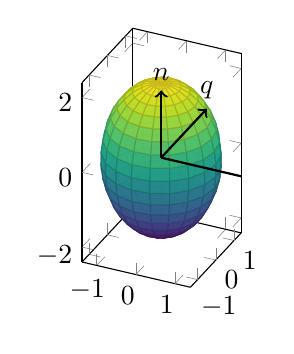
\begin{tikzpicture}
    \begin{axis}[
      %view={30}{20},      % camera angle
      %hide axis,
      axis equal image,
      samples=20,
      domain=0:360,
      y domain=-90:90
    ]
      % semi-axes of ellipsoid
      %\def\a{2.5}
      %\def\b{1.8}
      \def\c{2}
      \def\eps{0.3}
      \def\alph{1}
    
      % Draw the ellipsoid surface
      \addplot3[
        surf,
        %shader=interp,
        opacity=0.9,
        colormap/viridis
      ]
      (
        { \c*(1-\alph*\eps)*cos(x)*cos(y) },
        { \c*(1-\eps)*sin(x)*cos(y) },
        { \c*sin(y) }
      );
    
      % Coordinate axes with labels
      \draw[->, thick] (0,0,0) -- (3,0,0) node[anchor=west] {$p$};
      \draw[->, thick] (0,0,0) -- (0,2.5,0) node[anchor=south] {$q$};
      \draw[->, thick] (0,0,0) -- (0,0,1.8) node[anchor=south] {$n$};
    
    \end{axis}
    \end{tikzpicture}
    \caption{Prolate spheroid : $\varepsilon = 0.3, \alpha = 1$}
\end{figure}

For a spheroid parametrized as defined in section V,  $N_{npq} = 0$  and $N_{pqn} = - N_{qpn}$, $A = A_{pp} =A_{qq}$, $C = C_{pp} =C_{qq}$. 
Then, 
\begin{align}
    \dot \theta  = \cos \theta \sin \theta \frac{N_{pqn}F_b^2}{CA A_{nn}},
\end{align}
$A_{pp}, ...$ coefficients are all positive. Same for $C_{pp}, ...$. 
Then the orientation stability only depends on the sign of $N_{pqn}$, which itself depends on the shape of the spheroid ($i.e.$ prolate or oblate).
Indeed linearizing the previous equation around $\theta =0$ (or $\theta =\pi/2$) one gets,
\begin{align}
 \theta &= 0 \quad   \dot \theta  =  \theta \frac{N_{pqn}F_b^2}{CA A_{nn}} \quad \text{stable if $N_{pqn}< 0$}, \\
 \theta &= \frac{\pi}{2} \quad   \dot \theta  =  -\theta \frac{N_{pqn}F_b^2}{CA A_{nn}} \quad \text{stable if $N_{pqn}> 0$},.
\end{align}

For a spheroid with a small aspect ratio, using $C = 8\pi$, $A = 6\pi$, $A_{nn} = 6\pi$, and $N_{pqn} = \frac{29}{20}\pi \varepsilon$ (prolate if $\varepsilon >0$ ).
Then, $v = F_b/A$ where $v$ is the sedimenting velocity. 
This yields, 
\begin{equation}
  \dot \theta  = \cos \theta \sin \theta \frac{29}{160} \varepsilon v^2
\end{equation}
Our results differ from Cox by a factor of 3 (see his eq. 9.13). However, it appears that in eq. 9.11 he maybe omitted a factor of 1/3 (compare with his eqs. 7.3-7.5).
%Then if $N_{pqn}$ is positive ...


\subsection{Orientation of an ellipsoid}
We linearize the governing equations around the fixed points.
We know that $A_{pp}, ...$ coefficients are all positive. Same for $C_{pp}, ...$ coefficients. 

\subsubsection{$\{\theta = 0, \, \psi = 0\}$}
\begin{align}
    \dot \theta  &=  -\theta F_b^2 \frac{N_{qpn}}{C_{qq}A_{pp} A_{nn}} \quad \text{stable if $ N_{qpn}>0$ }, \\
    \dot \psi   &=  \psi F_b^2 \left(\frac{N_{pqn}}{C_{pp}A_{qq} A_{nn}}+\frac{N_{qpn}}{C_{qq}A_{pp} A_{nn}}\right)\text{stable if $\frac{N_{pqn}}{C_{pp}A_{qq} A_{nn}}  < -\frac{N_{qpn}}{C_{qq}A_{pp} A_{nn}}$}.
\end{align}
which implies $N_{pqn}<0$.

\subsubsection{$\{\theta = 0, \, \psi = \pi/2\}$}
\begin{align}
    \dot \theta  &=  \theta F_b^2 \frac{N_{pqn}}{C_{pp}A_{qq} A_{nn}}\quad \text{stable if $N_{pqn}<0$}, \\
    \dot \psi   &=  -\psi F_b^2 \left(\frac{N_{pqn}}{C_{pp}A_{qq} A_{nn}}+\frac{N_{qpn}}{C_{qq}A_{pp} A_{nn}}\right) \quad \text{stable if $\frac{N_{pqn}}{C_{pp}A_{qq} A_{nn}}  > -\frac{N_{qpn}}{C_{qq}A_{pp} A_{nn}}$}.
\end{align}
\subsubsection{$\{\theta = \pi/2, \, \psi = 0\}$}
\begin{align}
    \dot \theta  &=  +\theta F_b^2 \frac{N_{qpn}}{C_{qq}A_{pp} A_{nn}}\quad \text{stable if $ N_{qpn}<0$}, \\
    \dot \psi   &= -\psi F_b^2 \left(\frac{N_{npq}}{C_{nn}}\frac{1}{A_{pp} A_{qq}}\right)\quad \text{stable if $N_{npq}>0$}.
\end{align}
\subsubsection{$\{\theta = \pi/2, \, \psi = \pi/2\}$}
\begin{align}
  \dot \theta  &=  -\theta F_b^2 \frac{N_{pqn}}{C_{pp}A_{qq} A_{nn}}\quad \text{stable if $N_{pqn}>0$}, \\
  \dot \psi   &= -\psi F_b^2 \left(\frac{N_{npq}}{C_{nn}}\frac{1}{A_{pp} A_{qq}}\right)\quad \text{stable if $N_{npq}<0$}.
\end{align}

\subsubsection{Discussion}

The stability depends on the sign of $N_{qpn}$ and the sign of 
\begin{equation}
\frac{N_{qpn}}{C_{qq} A_{pp} A_{nn}} + \frac{N_{pqn}}{C_{pp} A_{qq} A_{nn}} .
\end{equation}
as well.
However, the values of $N_{qpn}$ and $N_{pqn}$ are not known for ellipsoidal particles of arbitrary shape.

\subsection{Ellipsoid close to a sphere}

In the following, we focus on an ellipsoid close to a spherical shape (see Section V), for which:

$$
N_{pqn} = \frac{29}{20}\pi \varepsilon, \quad
N_{qpn} = -\frac{29}{20}\pi \alpha \varepsilon, \quad
N_{npq} = \frac{29}{20}\pi (\alpha - 1)\varepsilon, \quad $$

$$
A_{pp} = 6\pi, \quad A_{qq} = 6\pi,  \quad A_{nn} = 6\pi ,
C_{pp} = 8\pi, \quad C_{qq} = 8\pi,  \quad C_{nn} = 8\pi .
$$

\subsubsection{$\{\theta = 0, \, \psi = 0\}$}

$\theta$ stable if $N_{qpn}>0$ $->$ $\alpha >0$ and $\varepsilon < 0$ or  $\alpha <0$ and $\varepsilon > 0$.\\
$\psi$ stable if $N_{pqn} < -N_{qpn}$ $->$ $\varepsilon < \alpha \varepsilon$ which requires  $1<\alpha$ if  $\varepsilon > 0$ or $1 > \alpha$ if $\varepsilon < 0$

Then the only possible configuration for which both conditions are satisfied is $\epsilon < 0$ and $0 <\alpha < 1$ (figure \ref{fig:example1})

\begin{figure}[h]
  \centering
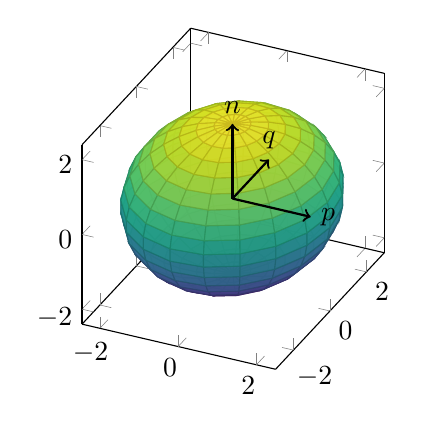
\begin{tikzpicture}
  \begin{axis}[
    %view={30}{20},      % camera angle
    %hide axis,
    axis equal image,
    samples=20,
    domain=0:360,
    y domain=-90:90
  ]
    % semi-axes of ellipsoid
    %\def\a{2.5}
    %\def\b{1.8}
    \def\c{2}
    \def\eps{-0.5}
    \def\alph{0.5}
  
    % Draw the ellipsoid surface
    \addplot3[
      surf,
      %shader=interp,
      opacity=0.9,
      colormap/viridis
    ]
    (
      { \c*(1-\alph*\eps)*cos(x)*cos(y) },
      { \c*(1-\eps)*sin(x)*cos(y) },
      { \c*sin(y) }
    );
  
    % Coordinate axes with labels
    \draw[->, thick] (0,0,0) -- (2,0,0) node[anchor=west] {$p$};
    \draw[->, thick] (0,0,0) -- (0,2,0) node[anchor=south] {$q$};
    \draw[->, thick] (0,0,0) -- (0,0,2) node[anchor=south] {$n$};
  
  \end{axis}
  \end{tikzpicture}
\caption{$\varepsilon = -0.5, \alpha = 0.5$}
\label{fig:example1}
\end{figure}

Ok since the plane $p,q$ (the broadest one) is perpendicular to gravity.

\subsubsection{$\{\theta = 0, \, \psi = \pi/2\}$}
$\theta$ stable if $N_{pqn} < 0$ $->$  $\varepsilon < 0$.\\
$\psi$ stable if $N_{pqn} > -N_{qpn}$ $->$ $\varepsilon > \alpha \varepsilon$ which requires  $1>\alpha$ if  $\varepsilon > 0$ or $1 < \alpha$ if $\varepsilon < 0$

This requires, $\varepsilon < 0$ and $\alpha >1$.
\begin{figure}[h]
  \centering
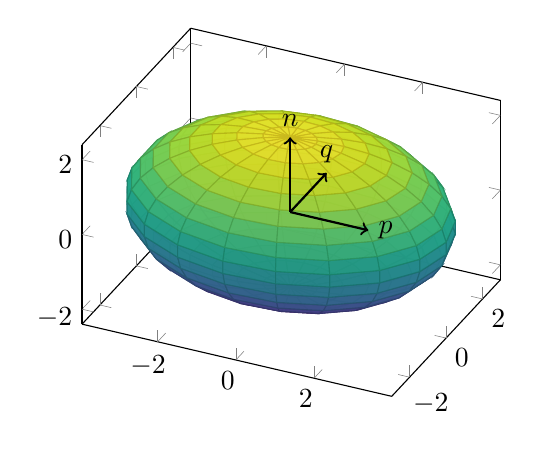
\begin{tikzpicture}
  \begin{axis}[
    %view={30}{20},      % camera angle
    %hide axis,
    axis equal image,
    samples=20,
    domain=0:360,
    y domain=-90:90
  ]
    % semi-axes of ellipsoid
    %\def\a{2.5}
    %\def\b{1.8}
    \def\c{2}
    \def\eps{-0.5}
    \def\alph{2}
  
    % Draw the ellipsoid surface
    \addplot3[
      surf,
      %shader=interp,
      opacity=0.9,
      colormap/viridis
    ]
    (
      { \c*(1-\alph*\eps)*cos(x)*cos(y) },
      { \c*(1-\eps)*sin(x)*cos(y) },
      { \c*sin(y) }
    );
  
    % Coordinate axes with labels
    \draw[->, thick] (0,0,0) -- (2,0,0) node[anchor=west] {$p$};
    \draw[->, thick] (0,0,0) -- (0,2,0) node[anchor=south] {$q$};
    \draw[->, thick] (0,0,0) -- (0,0,2) node[anchor=south] {$n$};
  
  \end{axis}
  \end{tikzpicture}
\caption{$\varepsilon = -0.5, \alpha = 2$}
\label{fig:example2}
\end{figure}

Ok since the plane $p,q$ (the broadest one) is perpendicular to gravity.

\subsubsection{$\{\theta = \pi/2, \, \psi = 0\}$}
$\theta$ stable if $ N_{qpn}<0$ $->$  $\alpha > 0$ and $\varepsilon > 0$ or  $\alpha < 0$ and $\varepsilon < 0$ .\\
$\psi$ stable if $N_{npq}>0$ or $(\alpha - 1)\varepsilon > 0$ which requires  $1 <\alpha$ if  $\varepsilon > 0$ or $1 > \alpha$ if $\varepsilon < 0$

which implies $0 > \alpha$ if $\varepsilon < 0$ or $1 <\alpha$ if  $\varepsilon > 0$ 

\begin{figure}[h]
  \centering
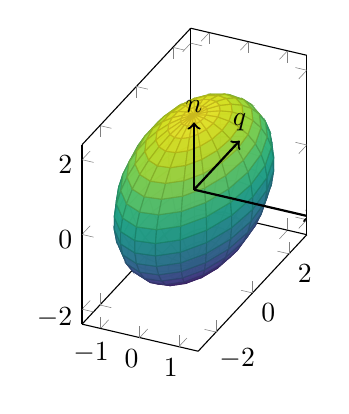
\begin{tikzpicture}
  \begin{axis}[
    %view={30}{20},      % camera angle
    %hide axis,
    axis equal image,
    samples=20,
    domain=0:360,
    y domain=-90:90
  ]
    % semi-axes of ellipsoid
    %\def\a{2.5}
    %\def\b{1.8}
    \def\c{2}
    \def\eps{-0.5}
    \def\alph{-0.5}
  
    % Draw the ellipsoid surface
    \addplot3[
      surf,
      %shader=interp,
      opacity=0.9,
      colormap/viridis
    ]
    (
      { \c*(1-\alph*\eps)*cos(x)*cos(y) },
      { \c*(1-\eps)*sin(x)*cos(y) },
      { \c*sin(y) }
    );
  
    % Coordinate axes with labels
    \draw[->, thick] (0,0,0) -- (3,0,0) node[anchor=west] {$p$};
    \draw[->, thick] (0,0,0) -- (0,2.5,0) node[anchor=south] {$q$};
    \draw[->, thick] (0,0,0) -- (0,0,1.8) node[anchor=south] {$n$};
  
  \end{axis}
  \end{tikzpicture}
  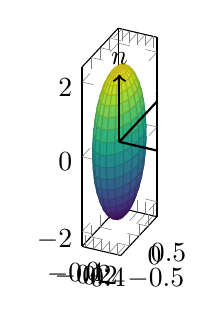
\begin{tikzpicture}
      \begin{axis}[
        %view={30}{20},      % camera angle
        %hide axis,
        axis equal image,
        samples=20,
        domain=0:360,
        y domain=-90:90
      ]
        % semi-axes of ellipsoid
        %\def\a{2.5}
        %\def\b{1.8}
        \def\c{2}
        \def\eps{0.5}
        \def\alph{1.5}
      
        % Draw the ellipsoid surface
        \addplot3[
          surf,
          %shader=interp,
          opacity=0.9,
          colormap/viridis
        ]
        (
          { \c*(1-\alph*\eps)*cos(x)*cos(y) },
          { \c*(1-\eps)*sin(x)*cos(y) },
          { \c*sin(y) }
        );
      
        % Coordinate axes with labels
        \draw[->, thick] (0,0,0) -- (3,0,0) node[anchor=west] {$p$};
        \draw[->, thick] (0,0,0) -- (0,2.5,0) node[anchor=south] {$q$};
        \draw[->, thick] (0,0,0) -- (0,0,1.8) node[anchor=south] {$n$};
      
      \end{axis}
      \end{tikzpicture}
\caption{(left): $\varepsilon = -0.5, \alpha = -0.5$, (right): $\varepsilon = 0.5, \alpha = 1.5$}
\end{figure}

Ok since the plane $(n,q)$ (the broadest one) is perpendicular to gravity.


\subsubsection{$\{\theta = \pi/2, \, \psi = \pi/2\}$}
$\theta$ stable if $N_{pqn}>0$ : $\varepsilon > 0$ .\\
$\psi$ stable if $N_{npq}<0$ or $(\alpha - 1)\varepsilon < 0$ which requires  $1 >\alpha$ if  $\varepsilon > 0$ or $1 < \alpha$ if $\varepsilon < 0$


thus requires, $1 >\alpha$ and  $\varepsilon > 0$

\begin{figure}[h]
  \centering
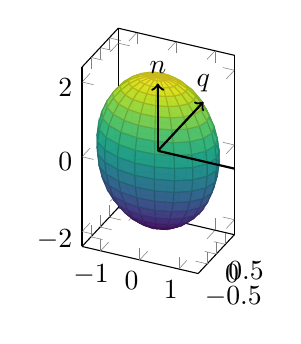
\begin{tikzpicture}
  \begin{axis}[
    %view={30}{20},      % camera angle
    %hide axis,
    axis equal image,
    samples=20,
    domain=0:360,
    y domain=-90:90
  ]
    % semi-axes of ellipsoid
    %\def\a{2.5}
    %\def\b{1.8}
    \def\c{2}
    \def\eps{0.5}
    \def\alph{0.5}
  
    % Draw the ellipsoid surface
    \addplot3[
      surf,
      %shader=interp,
      opacity=0.9,
      colormap/viridis
    ]
    (
      { \c*(1-\alph*\eps)*cos(x)*cos(y) },
      { \c*(1-\eps)*sin(x)*cos(y) },
      { \c*sin(y) }
    );
  
    % Coordinate axes with labels
    \draw[->, thick] (0,0,0) -- (3,0,0) node[anchor=west] {$p$};
    \draw[->, thick] (0,0,0) -- (0,2.5,0) node[anchor=south] {$q$};
    \draw[->, thick] (0,0,0) -- (0,0,1.8) node[anchor=south] {$n$};
  
  \end{axis}
  \end{tikzpicture}
  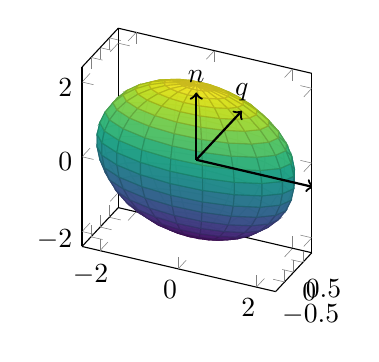
\begin{tikzpicture}
      \begin{axis}[
        %view={30}{20},      % camera angle
        %hide axis,
        axis equal image,
        samples=20,
        domain=0:360,
        y domain=-90:90
      ]
        % semi-axes of ellipsoid
        %\def\a{2.5}
        %\def\b{1.8}
        \def\c{2}
        \def\eps{0.5}
        \def\alph{-0.5}
      
        % Draw the ellipsoid surface
        \addplot3[
          surf,
          %shader=interp,
          opacity=0.9,
          colormap/viridis
        ]
        (
          { \c*(1-\alph*\eps)*cos(x)*cos(y) },
          { \c*(1-\eps)*sin(x)*cos(y) },
          { \c*sin(y) }
        );
      
        % Coordinate axes with labels
        \draw[->, thick] (0,0,0) -- (3,0,0) node[anchor=west] {$p$};
        \draw[->, thick] (0,0,0) -- (0,2.5,0) node[anchor=south] {$q$};
        \draw[->, thick] (0,0,0) -- (0,0,1.8) node[anchor=south] {$n$};
      
      \end{axis}
      \end{tikzpicture}
\caption{(left): $\varepsilon = 0.5, \alpha = 0.5$, (right): $\varepsilon = 0.5, \alpha = -0.5$}
\end{figure}

Ok since the plane $(n,p)$ (the broadest one) is perpendicular to gravity.



\subsection{Discussion}
In Bagheri's work, ellipsoidal particles are shown to adopt a stable orientation that maximizes their drag (broadest side perpendicular to gravity)
In other words, the particle aligns such that the projected surface area on a plane perpendicular to the direction of gravity is maximized.


\subsection{Slender-body limit}

In this section we consider a triaxial ellipsoid of semi-axis lengths ...
$$
N_{pqn} = , \quad
N_{qpn} = , \quad
N_{npq} = , \quad $$

$$
A_{pp} = 6\pi, \quad A_{qq} = 6\pi,  \quad A_{nn} = 6\pi ,
C_{pp} = 8\pi, \quad C_{qq} = 8\pi,  \quad C_{nn} = 8\pi .
$$


\bibliography{Bib/bib_bulles.bib}



\appendix


\end{document}
